\subsection*{A certificate for every point of the represented surface}
\label{sec:continuouscertificate}

The triangle rule defines a finite coverage problem. Its threshold tests do
not, by themselves, certify the intrinsic distance of every interior point
of a face. In particular, intrinsic balls on a folded surface need not be
convex. We give a separate sufficient certificate for the continuous
piecewise-flat surface represented by the mesh. This certificate permits
different contacts to witness coverage at different vertices and points.

Let $u_i(v)$ be a proved upper bound on the intrinsic mesh distance
$\dd(p_i,v)$, with contacts at mesh vertices. Write $u_k(v)$ for the $k$-th
smallest of these bounds. For a target triangle $T$, let $D_T$ be its longest
Euclidean edge and $m_T=\max_{v\in\operatorname{vert}(T)}u_k(v)$.

\begin{theorem}[whole-face coverage]\label{thm:wholeface}
Every point of $T$ belongs to at least $k$ open radius-$r$ intrinsic balls if
\[
                 m_T+D_T/\sqrt3<r.
\]
For closed balls the non-strict inequality suffices. If this holds for every
target face, the whole represented target remains covered after any $k-1$
contacts fail. The constant $1/\sqrt3$ is the smallest universal constant
possible when only the vertex bounds and longest edge are used.
\end{theorem}

\begin{proof}
Every function $\dd(p_i,\cdot)$ is $1$-Lipschitz. Their $k$-th order statistic
$g_k$ is also $1$-Lipschitz: moving a point by $h$ increases each of the $k$
distances below the old $k$-th distance by at most $h$, and reversing the
points gives the opposite inequality. Coordinatewise upper bounds preserve
order statistics, so $g_k(v)\le u_k(v)$.

For $x=\sum_{j=1}^3\lambda_jv_j\in T$, the barycentric variance identity gives
\[
 \sum_j\lambda_j|x-v_j|^2
 =\sum_{i<j}\lambda_i\lambda_j|v_i-v_j|^2
 \le\frac{D_T^2}2\left(1-\sum_j\lambda_j^2\right)
 \le D_T^2/3.
\]
At least one vertex therefore has $|x-v_j|\le D_T/\sqrt3$. The straight
segment inside the face is a permissible surface path, so
$g_k(x)\le g_k(v_j)+\dd(v_j,x)\le m_T+D_T/\sqrt3$.
This proves both coverage assertions. At each point at least $k$ distinct
contacts cover it; deleting $k-1$ leaves a survivor.

For sharpness, take $k=1$ and put contacts at the vertices of an equilateral
triangle of side $D$. The nearest-contact distance is zero at all vertices
and $D/\sqrt3$ at the centre. Any smaller constant would certify a radius
strictly below the centre's distance.
\end{proof}

\begin{corollary}[bounded location and radius error]\label{cor:errorbudget}
Suppose each actual contact lies within $\varepsilon$ of its nominal
location in the same intrinsic metric, and its actual footprint radius is
at least $r-\delta$, where $\varepsilon,\delta\ge0$. The sufficient open-ball
test becomes $m_T+D_T/\sqrt3+\varepsilon+\delta<r$.
\end{corollary}
\begin{proof}
The triangle inequality increases each contact distance by at most
$\varepsilon$; decreasing every radius by at most $\delta$ gives the stated
margin. Apply Theorem~\ref{thm:wholeface}.
\end{proof}

\paragraph{Constructing genuine distance upper bounds.}
We obtain these bounds from explicit mesh-edge paths. Treat the stored
binary64 coordinates as exact dyadic numbers and fix a length quantum
$h=2^{-20}$\,mm. For every edge with exact squared length $s_e$, compute
\[
             w_e=\left\lceil\sqrt{s_e/h^2}\right\rceil
\]
using integer arithmetic and an integer square root. Its surface length is
at most $hw_e$. Dijkstra's algorithm with these integer weights returns a
path whose length bound is the exact number $h\sum_e w_e$. Conversion to
binary64 is rounded outward, with an exact rational check. These numbers
are therefore upper bounds on intrinsic mesh distances, even though the
shortest intrinsic path can cross face interiors and be shorter.

The search is truncated at $16$\,mm for efficiency. An unreached vertex is
assigned the conservative bound $(V-1)h\max_e w_e$, justified by a simple
path in the connected $V$-vertex edge graph. It is never assigned zero or
declared covered because it was unreached. Finally, putting $t=r-m_T$, the
whole-face decision is the exact rational comparison $t>0$ and
$D_T^2<3t^2$; closed-ball coverage uses non-strict signs. An unresolved face
may already be covered and is not an uncovered-point certificate.

The target is the stored list of \patchTris{} faces selected by the earlier
patch construction. We certify their union; the floating-point selection
of that list is not a certificate that it equals an exact $35$\,mm intrinsic
disk. Likewise, a certificate on this mesh does not bound discrepancies
between the template and a patient's cortex.

\begin{table}[t]
\centering
\caption{Whole-face certificates using upward path bounds. Every entry
certifies all \patchTris{} target triangles as continuous piecewise-flat
faces. Contact sets are prefixes of the stored free-contact sequence;
these sufficient examples do not establish globally minimum counts.}
\label{tab:continuouscertificates}
% Generated by make_certified_figure.py
\begin{tabular}{rrrr}
\toprule
Contacts & Radius (mm) & Multiplicity $k$ & Failures tolerated \\
\midrule
64 & 9 & 1 & 0 \\
80 & 8 & 1 & 0 \\
112 & 10 & 2 & 1 \\
128 & 9 & 2 & 1 \\
160 & 8 & 2 & 1 \\
\bottomrule
\end{tabular}

\end{table}

Table~\ref{tab:continuouscertificates} and Fig.~\ref{fig:certifiedmesh} report
the new computation. The machine-readable audit record in the repository
contains exact input hashes. The displayed contact counts are drawn
from the prescribed set $64,66,80,96,112,128,160$; no claim is made about
untested intermediate counts. Their certificates are independent of the
good-cover hypothesis needed for the nerve theorem. The previously reported
triangle-rule results, such as 66 contacts at $8$\,mm, remain results of
that finite rule and are not promoted to the stronger whole-face guarantee.

\begin{figure}[t]
\centering
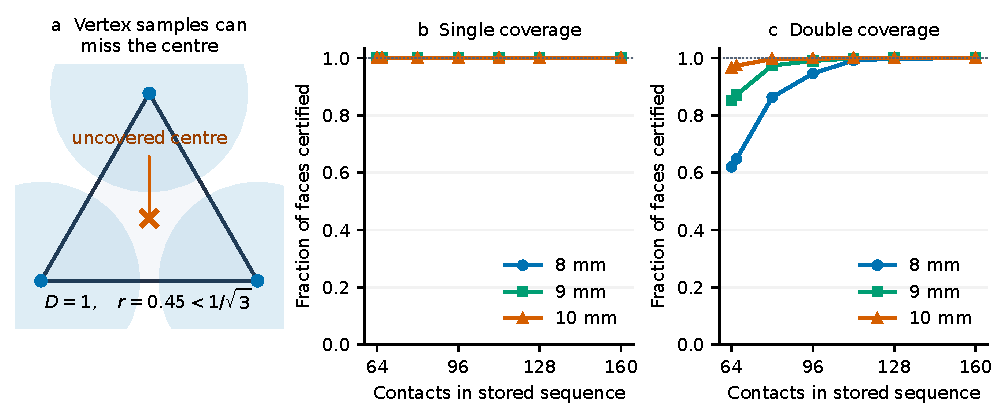
\includegraphics[width=\textwidth]{certified_mesh.pdf}
\caption{From vertex samples to whole-face coverage. (a) Three contacts at
the vertices of a unit equilateral triangle cover all vertices at radius
$0.45$, while leaving its centre uncovered. The sharp universal vertex
margin is $D/\sqrt3$. (b,c) Fraction of the template target faces passing the
rigorous test for single and double coverage. A value of one certifies every
point of the represented target. Lower fractions indicate unresolved faces,
not a measured uncovered area.}
\label{fig:certifiedmesh}
\end{figure}
